%--------------------------------------------------------------------------------------------------------------------------------
%build
%--------------------------------------------------------------------------------------------------------------------------------
\subsection{Build}
	\subsubsection{Syntax}
		\texttt{build([argument list])}
	
	\begin{phygdescription}
	
		{Builds initial graphs. The arguments of \texttt{build} specify the number of graphs 
		to be generated, and whether the build is based on \textit{distance} or \textit{character} 
		methods. The distance options \texttt{rdWag} and \texttt{wpgma} have a time complexity 
		of $O(n^2)$, while \texttt{dWag} and \texttt{nj} have a complexity of $O(n^3)$. Distance 
		methods are considerably faster (lower constant factor), but approximate, compared to 
		character-based methods. Refinement, in the form of branch swapping (\texttt{none}, 
		\texttt{otu}, \texttt{spr}, and \texttt{tbr}) can be specified within the command for distance 
		builds. Refinement for character-based Wagner builds occurs after the \texttt{build} 
		process through \texttt{swap} and other refinement commands. Given the large time 
		complexity, distance refinement is usually not worth the effort \citep{Wheeler2021}. 
		\texttt{build} does not replace graphs previously 
		stored in memory.}
		
	\end{phygdescription}
		
	\subsubsection{Arguments}

	\begin{description}
	
		\item[block] Performs independent builds for each `block' of data. If this option 
		is not specified, the builds are performed combining all the data. Builds are performed 
		according 	to the other options, i.e. \texttt{character} or \texttt{distance}. The resulting 
		tree or \texttt{graph} is reconciled using the \texttt{eun} or \texttt{cun} commands. The 
		reconciled graph is resolved into display trees via the \texttt{displayTrees}, \texttt{first}, 
		and \texttt{atRandom} options. This option is especially useful for softwired network 
		search. Associated arguments of \texttt{block} include:
				
		\begin{description}
					
			\item[cun] Reconciles \textbf {block} trees into a Cluster-Union-Network 
			\citep{Baroni2005} before resolution into display trees via \texttt{displayTrees} 
			and its associated arguments.
	
			\item[displayTrees[:INT]] When the option \texttt{block} is specified, this variable 
			returns $n$ display trees specified by this optional argument. If the number of 
			display trees is not specified, up to $2^{63}$ may be returned.
				
			\begin{description}
				
				\item[atRandom] When the option \texttt{block} is specified, this variable 
				returns the number of display trees as specified by the integer value in 
				\texttt{displayTrees[:INT]}, where trees are produced by resolving network 
				nodes uniformly at random. Compare with \texttt{first}.
				
				\item[first:INT] When the option \texttt{block} is specified, this variable specifies 
				that the first number of displays tree resolutions, as specified by the integer 
				value, are chosen for each input graph. Compare with \texttt{atRandom}.
				
			\end{description}

			\item[eun] Reconciles block trees into a Edge-Union-Network \citep{MiyagiandWheeler2019, 
			Wheeler2022} before resolution into display trees via \texttt{displayTrees} and its associated 
			arguments.
						
			\item[graph] When the option \texttt{block} is specified, this variable returns the 
			reconciled graph as specified by \texttt{eun} or \texttt{cun}. The graph may be 
			altered to ensure that it is a `phylogenetic' graph sensu \cite{Moretetal2005}.
			
		\end{description}			
		
		\item [character] Performs random addition sequence Wagner \citep{Farris1970} builds 
		($O(n^2)$) for tree construction. If the graphtype is specified as softwired or hardwired, 
		the resulting trees are rediagnosed as softwired graphs. This is 
		the default method for tree construction.
		
		\item [distance] Causes a pairwise distance matrix to be calculated ($O(n^2)$) and used 
		as a basis for distance tree construction. Specifies how the builds are refined (\texttt{none}, 
		\texttt{otu}, \texttt{spr}, \texttt{tbr}), as well as how the tree is constructed (\texttt{dWag}, 
		\texttt{nj}, \texttt{rdWag}, \texttt{wpgma}). Distance trees are subsequently rediagnosed 
		as character trees and returned for further analysis. Associated arguments of \texttt{distance} 
		include:
					
		\begin{description}
		
			\item[dWag] Performs distance Wagner build as in \citep{Farris1972} choosing the 
			`best' taxon to 
			add at each step, yielding a single tree. This method has a time complexity of $O(n^3)$.

			\item[nj] Performs Neighbor-Joining distance build \citep{Saitou1987}, yielding a single 
			tree. This method has a time complexity of $O(n^3)$.

			\item[none] No refinement (\texttt{otu}, \texttt{spr}, \texttt{tbr}) is performed after 
			distance builds. \texttt{none} is the default refinement method.
						
			\item[otu] Specifies that OTU refinement \citep{Wheeler2021} is performed 
			after distance builds.
			
			\item[rdWag] Performs random addition sequence distance Wagner builds 
			\citep{Farris1972,Wheeler2021}, yielding multiple trees determined by the 
			argument \texttt{replicates}. This method has a time complexity of $O(m \times n^2)$
			for $m$ replicates and $n$ taxa.
			
			\begin{description}
				
				\item[best:INT] Applies only to \texttt{rdWag}. Specifies the number of trees 
				retained after \texttt{rdWag} builds, selecting the best trees in terms of distance 
				cost. The options can be used to reduce the number of trees retained.  
				
			\end{description}
			
			\item[spr] Specifies that SPR refinement \citep{Dayhoff1969} is performed 
			after distance builds.

			\item[tbr] Specifies that TBR refinement \citep{Farris1988, swofford1990a} 
			is performed after distance builds.
		
			\item[wpgma] Performs Weighted Pair Group Method with Arithmetic Mean 
			distance build \citep{SokalandMichener1958}, yielding a single tree. This method 
			has a time complexity of $O(n^2)$.
			
		\end{description}

		\item [replicates:[INT]] Applies to \texttt{rdWag} and \texttt{character}. Specifies the 
		number of random addition sequences to be performed, as indicated by the integer 
		value. By default 10 random addition sequences are performed.
		
		\item[return:[INT]] Applies to \texttt{rdWag} and \texttt{character}. This limits the 
		number of Wagner trees returned for further analysis, to the value as specified 
		by the integer. By default all graphs that are built are returned, unless limited 
		by \texttt{best} in distance analysis. Limiting the number of returned trees 
		(as opposed to simply generating that number) can result in a larger memory 
		footprint.
			
	\end{description}		

	\subsubsection{Defaults}
		\texttt{build(character, replicates:10)} By default, \phyg will build 10 graphs using 
		a random addition of sequences for each of them.
		
	\begin{example}
	
		\item{\texttt{build(replicates:100)} \\
		Builds 100 graphs using a random addition sequence (the default) for each of them.}
		
		\item{\texttt{build(character, block, graph, cun, displaytrees:5, atrandom)}\\
		Builds 10 (the default) random addition sequence character Wagner builds, for each 
		block of data. The graph is reconciled into a Cluster-Union-Network, before resolution 
		into 5 display trees. The trees are produced by resolving the network nodes 
		uniformly at random.}
		
		\item{\texttt{build(distance, dWag, nj, wpgma)} \\ 
		Builds a single `best' distance Wagner build, a Neighbor-Joining tree, and a 
		WPGMA tree. As the option \texttt{block} is not specified, the distance trees 
		are built using all the data. A total of three trees is returned.}
		
		\item{\texttt{build(distance, dWag, replicates:1000, best:10)}\\
		Builds 1000 distance Wagner builds and returns 10 of the lowest cost distance trees.
		The best trees are chosen arbitrarily, but consistently--the first 10 with the lowest cost.}
	
		\item{\texttt{build(distance, rdwag, block, eun, displaytrees:3)}\\
		Builds 10 random addition sequence Wagner builds for each `block' of data. The graph 
		is reconciled into a Edge-Union-Network, before resolution into the 3 display trees. 
		The trees are produced by resolving the network nodes.}
		
		\item{\texttt{build(distance, block, rdWag, wpgma, replicates:100, best:10, otu)}\\
		Builds 100 random addition sequence distance Wagner builds and a wpgma tree. 
		OTU swapping is performed on the 10 of the lowest cost random addition 
		sequence Wagner trees. These distance searches, and subsequent refinements are 
		performed on each block of data.}
		
	\end{example}

%--------------------------------------------------------------------------------------------------------------------------------
%fuse
%--------------------------------------------------------------------------------------------------------------------------------
\subsection{Fuse}
	\subsubsection{Syntax}
		\texttt{fuse([argument list])}
		
	\begin{phygdescription}
	
		{Performs Tree Fusing \citep{goloboff1999, moilanen1999, moilanen2001} on the graphs
		in memory. \texttt{fuse} operates on a collection of graphs performing reciprocal graph 
		recombination between pairs of graphs. Non-identical subgraphs with identical leaf sets 
		are exchanged between graphs and the results evaluated. This process of exchange 
		and evaluation continues until no new graphs are found. This can be used in concert 
		with other options to perform a Genetic Algorithm refinement \citep{Holland1975}. The 
		behavior of \texttt{fuse} can be modified by the use of options specifying SPR and 
		TBR-like rearrangement of the combination process.}
		
	\end{phygdescription}
	
	\subsubsection{Arguments}
	
	\begin{description}
	
		\item [all]  During branch swapping-type operations, all rearrangements are tried before 
		choosing a new graph. 
		
		\item [best] Specifies the method for tree selection, which in this case returns the best 
		graphs found during fuse operations.		
		
		\item [keep:INT] Limits the number of returned graphs to the integer value specified. 
		
		\item [none] No branch swapping is performed during the fuse. This is the default.
		
		\item [noReciprocal] Turns off \texttt{reciprocal} (see below).
		
		\item [once] Performs a single round of fusing on input graphs and returns the resulting 
		graphs. Alternatively (and by default) fusing continues recursively until no new graphs 
		are found.
		
		\item [pairs:INT] Limits the number of graphs to be fused to the number of pairs as 
		specified by the integer value (as oppose to $\binom{m}{2}$ for $m$ graphs).
		
		\begin{description}
			
			\item [atRandom] Chooses graphs to fuse uniformly at random when \texttt{pairs} is 
			specified. 
			
		\end{description}
		
		\item [reciprocal] By default, fuse takes a subgraph of one graph in a pair and replaces the 
		corresponding subgraph in the other.  This argument results in the exchange and evaluation 
		of graphs in both directions---roughly doubling both the time and memory footprint.
		
		\item [spr[:INT]] Causes the exchanged subgraphs to be tried at multiple positions (up to 
		$n$ edges away from their initial positions, where $n$ equals the integer value).
		
		\item [steepest] During branch swapping-type operations, if a better graph is found, swapping 
		shifts greedily to that graph. This is the default if swapping is specified.
		
		\item [tbr[:INT]] Causes the exchanged subgraphs to be tried at multiple positions (up to 
		$n$ edges away from their initial positions) where $n$ equals the integer value. TBR-style 
		rerooting of the exchanged components occurs.
		
		\item [unique] Specifies the method for tree selection, which in this case returns all unique 
		graphs found during fuse operations.	
		
	\end{description}	
	
	\subsubsection{Defaults}
		\texttt{fuse(best, none, reciprocal)} By default, \phyg keeps all the best graphs found, 
		and continues fusing until no new graphs are found. No branch swapping style rearrangements 
		are performed. The exchange and evaluation of graphs occurs in a reciprocal manner. 
			
	\begin{example}
	
		\item{\texttt{fuse(best, once)}\\Fuses input graphs and returns best graphs after a single 
		round of fusing. No branch swapping style rearrangements are performed and the exchange 
		and evaluation of graphs occurs in a reciprocal manner (the default).}
		
		\item{\texttt{fuse(tbr, keep:10)} \\Fuses input graphs and performs TBR-style replacement 
		and rerooting of pruned components returning up to 10 best cost graphs. The exchange 
		and evaluation of graphs occurs in a reciprocal manner (the default).}
		
		\item{\texttt{fuse(spr:3, pairs:5, unique)} \\Fuses input graphs and performs SPR-style swapping, 
		with the exchange of subgraphs being tried at multiple positions up to 3 edges away from their 
		initial position. The number of graph pairs to be fused is limited to 5. All unique graphs found
		during this operation are returned. The exchange and evaluation of graphs occurs in a reciprocal 
		manner (the default)}.
		
	\end{example}

%--------------------------------------------------------------------------------------------------------------------------------
%read
%--------------------------------------------------------------------------------------------------------------------------------
	
\subsection{Read}
\label{subsec:read}
	\subsubsection{Syntax}
		\texttt{read(argument list)}
			
	\begin{phygdescription}
		{Imports file-based information, including data files and graph files. \texttt{read} 
		commands must contain an input file (\texttt{STRING}). Supported data formats 
		include FASTA, FASTC and TNT files, and graph formats include Dot, eNewick, %Fenewick (not yet implemented) 
		and Newick. Filenames must be included in quotes. Filenames must include the 
		appropriate suffix (e.g. .fas, .ss, .mat). The exclusion of these suffixes will result 
		in an error. The filename must match exactly, including capitalization. \phyg will 
		attempt to recognize the type of input and parse appropriately. Otherwise, the 
		type of file can be explicitly indicated, using one of arguments below. The argument 
		is followed by a colon (`:') and the data file name(s), enclosed in quotes, and 
		separated by commas. It is possible to import more than one data file on the 
		same input line of the command script, but only of the same data type. Reading 
		in files of different data types, e.g. amino acid and nucleotide in the same command, 
		will result in an error. Prepending the file type prevents any ambiguity when the file 
		is parsed (e.g. \texttt{read(nucleotide:"Chel.fas")}). If the data type is not specified, 
		it is important to verify that the data was interpreted properly (using the command 
		\texttt{report("STRING", data)} or by checking the output display in the 
		\textit{Terminal} window). \texttt{read} can also use wildcard expressions 
		(`*' and `?'), which can be useful when reading in multiple files of the 
		same type. For example, \texttt{read(preaminoacid:"*.fas*")} imports all files of the 
		FASTA format in the current directory (in this case this will include files that end 
		in both .fas and .fasta). This files will be interpreted as prealigned amino acid
		sequences. Terminal names should not have spaces in the imported 
		data file, otherwise the names can be incorrectly interpreted by the program.} 
	\end{phygdescription}

	\subsubsection{Arguments}
	
	\begin{description}
	
		\item [aminoacid:STRING] Specifies that the file contents are parsed as IUPAC 
		coded amino acid data in FASTA \citep{PearsonandLipman1988} format. Sequence 
		gaps are removed.

		\begin{tcolorbox}[enhanced,fit to height=3cm,
  		colback=JungleGreen!40!black!2!white,colframe=JungleGreen!70!black,title=Note,
  		drop fuzzy shadow]
  		\phyg recognizes the characters `\textbf{x}' as representing any IUPAC character in 
		amino acid data, and `\textbf{n}' as representing any nucleotide base in nucleotide 
		sequence data files. A question mark character (`\textbf{?}') represents either an 
		`\textbf{x}' or a gap character `\textbf{-}' in amino acid data or an `\textbf{n}' or a 
		`\textbf{-}' nucleotide sequence data.
		\end{tcolorbox}

		\item [block:STRING] Specifies that the string contains block information. Each line 
		contains the new block name followed by names of input files to be assigned to that 
		data block. Blocks are initially named as the input file name with ``\#0'' appended. 
		In the example below, data from files ``b'' and ``c'' will be assigned to block ``a''. 
		There can be no spaces in file or block names. This argument is only intended for 
		use with softwired networks. Characters in the same block have the same display 
		tree in a softwired network \citep{WheelerandWashburn2023}.
			
			\begin{quote}
			\texttt{"a" "b\#0" "c\#0"}
			\end{quote}
	
		\item [dot:STRING] Specifies that the file contains a graph in `dot' format for use with 
		graph rendering software such as \href{https://en.wikipedia.org/wiki/Graphviz}{GraphViz}.
			
		\item [enewick:STRING] Specifies that the file contains Enhanced Newick format graph(s) 
		as specified here \citep{Cardonaetal2008}. 
			
		\item [exclude:STRING] Specifies that the file contains the names of terminal taxa to be 
		excluded from an analysis. Taxa appear in the form of a list, with a single taxon per 
		line. Thus, taxa not included in the list and present in input files, will be included in 
		analysis. Compare with \texttt{include}.
			
		\item [fasta:STRING] Ensures that file contents are parsed in FASTA \citep{PearsonandLipman1988}
		format. This is used for single character sequences such as binary streams, IUPAC 
		nucleotide and amino acid sequence data. Sequence gaps are removed.
			
		\item [fastc:STRING] Ensures that file contents are parsed in FASTC \citep{WheelerandWashburn2019}
		format. This is used for multi-character sequences such as gene synteny, developmental, 
		or linguistic data.   Sequence gaps are removed.
			
%		\item [fenewick:STRING] Specifies that the file contains Forest Enhanced Newick format graph(s) 
%		specified \href{https://www.github.com/wardwheeler/euncon}{here} \citep{Wheeler2022}.
%		Not yet implemented.
		
%		\item [gapopening:] Not yet implemented.

%		\item [hugeseq:] Only internal---used for testing purposes.
	
		\item [include:STRING] Specifies the names of terminal taxa to be included in the analysis. 
		Taxa appear in the form of a list, with a single taxon per line. It is possible to specify 
		terminals that have no data. This may be done in order to diagnose a large graph on 
		partial data. If there are no data for a leaf taxon, a warning will be printed to \texttt{stderr}. 
		Taxa not included in this list, but present in the inputted data files, will be excluded from 
		the analysis. Compare with \texttt{exclude}.
			
		\item [newick:STRING] Specifies that the file contains Newick format graph(s) as specified 
		\href{https://evolution.genetics.washington.edu/phylip/newick_doc.html}{here}.
			
		\item [nucleotide:STRING] Ensures that file contents are parsed as IUPAC coded nucleotide 
		data in FASTA \citep{PearsonandLipman1988} format. Sequence gaps are removed.
		
		\begin{tcolorbox}[enhanced,fit to height=3.5cm,
  		colback=JungleGreen!40!black!2!white,colframe=JungleGreen!70!black,title=Note,
  		drop fuzzy shadow]
  		Sequences can be divided into smaller fragments using an assigned character (default 
		`\textbf{\#}'). This character can be chosen by the user (unlike in POY, where the pound sign 
		(`\textbf{\#}') was the only character used to partition datasets). Each fragment is treated as 
		an individual character. When partitioning the data in this way, the number of partitions must 
		be the same across homologous sequences. The character should be set with the command 
		\texttt{set:partitioncharacter} (see Section \ref{subsec:set}).
		\end{tcolorbox}
			
		\item [preaminoacid:STRING] Specifies that the file contents are parsed as IUPAC coded 
		amino acid data in prealigned FASTA \citep{PearsonandLipman1988} format. Gap characters 
		(``-'') in the sequences are maintained and alignment correspondences are not re-examined.
		Prealigned amino acid sequence data \textit{must} be of the same length.
	
		\item [prefasta:STRING] Specifies that the sequences are prealigned in a FASTA format, 
		leaving gap characters (``-'') in the sequences and alignment correspondences are not 
		re-examined. This option exists to ensure proper parsing (and in case auto-format detection 
		is incorrect). Prefasta files can include any single character element such as nucleotide 
		sequence data, binary data or IUPAC amino acid sequences. Prealigned FASTA files 
		\textit{must} be of the same length. 
			
		\item [prefastc:STRING] Specifies that the sequences are prealigned in a FASTC format, 
		leaving gap characters (``-'') in the sequences and alignment correspondences are not 
		re-examined. This option exists to ensure proper parsing (and in case auto-format detection 
		is incorrect). Prealigned FASTC files \textit{must} be of the same length.
		
%		\item [prehugeseq:] Only internal---used for testing purposes.			
		
		\item [prenucleotide:STRING] Ensures that file contents are parsed as IUPAC coded 
		nucleotide data in FASTA \citep{PearsonandLipman1988} format, leaving gap characters 
		(``-'') in the sequences and alignment correspondences are not re-examined. Prealigned 
		nucleotide sequence data \textit{must} be of the same length.
		
		\item [rename:STRING] Replaces the name(s) of specified terminals in the file. This 
		command allows for substituting taxon names and can help merge multiple datasets without 
		modifying the original data file. The file contains a series of lines, each of which contains at 
		least two strings---these strings equate to synonyms separated by spaces. The first string 
		(input taxon name) will replace the second and all subsequent strings (taxon names) on 
		that line. The \texttt{rename} function can also be specified as a command, see \texttt{rename}
		(Section \ref{subsec:Rename}) for more detail and examples.
					 
		\item[STRING] Reads the file specified in the path included in the string argument. A path 
		can be absolute or relative to the current working directory. The file type is recognized
		automatically, but as mentioned previously, this should be confirmed.

		\item [tcm:STRING] This refers to a file containing a custom-alphabet matrix that 
		specifies varying costs among alphabet elements in a sequence. The elements in 
		the alphabet can be letters, digits, or both.
		The \texttt{tcm} contains two parts: the first line of the file contains the alphabet elements 
		separated by a space and the transformation cost matrix, which follows below. The dash 
		character representing an insertion/deletion or indel character is not specified on the first 
		line of the file, but added to the alphabet automatically. The second part is the \texttt{tcm}, 
		which is a square matrix with $n + 1$ elements ($n$ is the size of the alphabet). 
		The positions from left to right and top to bottom in this matrix correspond to the sequence 
		of the elements as they are listed in the alphabet. An extra rightmost column and lowermost
		row correspond to indel (gap) costs to and from alphabet elements. At present, this matrix 
		must be symmetrical, but not necessarily metric. Non-metric tcms can yield unexpected 
		results. Transformation costs must be integers. If real values are desired, a character can 
		be weighted with a floating point value factor. \\
		
		For a sequence with four elements alpha, beta, gamma and delta and an indel cost of 5 
		for all insertion deletion transformations, a valid custom alphabet file is provided below:
		\\
		\begin{equation*}
		%\nolabel
		\begin{array}{lllll}
		alpha & beta & gamma & delta &  \\
		0 &   2 &  1 &   2 &   5 \\
		2 &   0 &  2 &   1 &   5 \\
		1 &   2 &  0 &   2 &   5 \\
		2 &   1 &  2 &   0 &   5 \\
		5 &   5 &  5 &   5 &   0
		\end{array}
		\end{equation*} 
		\\
		
		In this example, the cost of transformation of \texttt{alpha} into \texttt{beta} is \texttt{2},
		and cost of a deletion or insertion of any of the four elements is \texttt{5}.

		\item [tnt:STRING] Ensures that file contents are parsed in TNT \citep{Goloboffetal2008} 
		format. Not all TNT data commands are currently supported. To ensure that the file is 
		correctly parsed, the file must begin with \texttt{xread}, followed by an optional comment 
		in single quotes (`this is a comment'), followed by the number of characters and taxa. The 
		data follow on a new line. Taxon names are followed by character state data. Data can be in 
		multiple blocks (interleaved) or in sequential format. These interleaved blocks can consist 
		of a series of single character states without spaces between them, or multiple (or single) 
		character states (e.g. \textbf{alpha}) with space between the individual codings. Blocks 
		must be of all one type (i.e. single character codings without spaces, or multi-character 
		separated by spaces). The data block \textit{must} be followed by a single semicolon 
		(`;') on its own line.\\
			
		The character settings (i.e. \texttt{ccode} commands) follow the data block, beginning 
		on a 	new line. These character settings always terminate with a semi-colon (`\texttt{;}'). 
		These settings include: activate (`\texttt{[}') or deactivate (`\texttt{]}'); make additive/ordered 
		(`\texttt{+}') or non-additive/unordered (`\texttt{-}'); apply step-matrix costs (`\texttt{(}') with 
		scopes (e.g. \texttt{cc + 10 12;} and  \texttt{cc (.; costs 0 = 0/1 1 0/2 2 0/3 3 0/4 4 1/2 1 
		1/3 2 1/4 3 2/3 1 2/4 2 3/4 1;}) including abbreviated scopes (`\texttt{cc -.;}'). There may 
		be multiple character setting statements in a single line. Character settings must be 
		followed by \texttt{proc/;} on its own line. \texttt{PhyG} will not process
		any file contents that follow \texttt{proc/;}.\\
		  
		 Additive/ordered character states must be numbers (integer or floating point). Ranges 
		 for continuous characters are specified with a dash within square brackets (e.g. 
		 \texttt{[1-2.1]}). Character state polymorphism are specified in square brackets without 
		 spaces for single character states (e.g. \texttt{[03]}), and with spaces for multi-character 
		 states.\\
		  
		 Dashes in multi-character states (e.g. \texttt{Blue-ish}) are treated as part of the character 
		 state specification.
		 %If the user wishes that dashes be treated as missing data, the file must be edited to 
		 %reflect this by replacing the dashes that are to be treated as missing data with question 
		 %marks (`?').
		 \\
		  
		  Example file:
		  	\begin{quote}
			  	\texttt{xread\\
				  	`An example TNT file' 8 5\\
				  	A 000\\
				  	B a14\\
				  	C b22\\
				  	D ?33\\
				  	E d[01]4\\}
			  	
			  	\texttt{A Blue-ish -\\
				  	B Green-ish OneFish\\
				  	C Rather-Red TwoFish\\
				  	D Almost-Cyan RedFish\\
				  	E Orange-definitely BlueFish\\}
					
				\texttt{A 5.2 - ?\\
					 B 5.3 0.3 1.1\\
					 C 3.2 0.1 1.1\\
					 D 5.2 1.1 0.1\\
					 E 5.1 1.1 0.1\\
				  	;\\
				  	cc .;\\
				  	cc + 2;\\
				  	proc/;\\}
			  \end{quote}
			  
	\end{description}	
		
	\subsubsection{Defaults}
		\texttt{read("fileName")} reads data within the data file ``fileName'' and attempts to 
		recognize the file type and parse accordingly. The assumed file type is printed to 
		\texttt{stderr} for verification.
		
	\begin{example}
	
		\item{\texttt{read(nucleotide:"/Users/UserName/Desktop/phyg/metazoa.fas", 
		tcm:"sg1t4.mat")}\\ Reads the file ``\textbf{metazoa.fas}'' located in the path 
		\textbf{/Users/UserName/Desktop/phyg/}, parsing it as nucleotide sequence 
		data. The information in the transformation cost matrix \textbf{sg1t4.mat} 
		is applied to this imported sequence data.}
		
		\item{\texttt{read(prefasta:"myDnaSequenceFile.fas")}\\ Reads sequence data from 
		``\textbf{myDnaSequenceFile.fas}'' as prealigned data.}
		
		\item{\texttt{read(include:"IncludeTaxa.txt")}\\ Reads a list of taxa in the file 
		``\textbf{IncludeTaxa.txt}'' to be included in the analysis. All other taxa not included 
		in this list, but present in the inputted data files, will be excluded from the analysis.}
		
		\item{\texttt{read(rename:"RenameFile.txt")}\\ Reads the file ``\textbf{RenameFile.txt}'' 
		that contains a list synonyms, where the name of the item listed first will be substituted 
		for all the subsequently listed names. }
		
		\item{\texttt{read(newick:"squamata\_run1.tre", "squamata\_run2.tre")}\\ Reads the
		Newick graph files ``\textbf{squamata\_run1.tre}'' and ``\textbf{squamata\_run2.tre}.}
		
	\end{example}
		
%--------------------------------------------------------------------------------------------------------------------------------
%reblock
%--------------------------------------------------------------------------------------------------------------------------------
\subsection{Reblock}
\label{subsec:reblock}
	\subsubsection{Syntax}
		%\texttt{reblock("newBlockName", "inputFile0", "inputFile1",...)}
		\texttt{reblock(STRING list)}
	
	\begin{phygdescription}
		{Assigns input data to `blocks' that will follow the same display tree when optimized
		as `softwired' networks. By default, each input data file is assigned its own block with 
		the name of the input file. The command \texttt{read(block)} (see Section \ref{subsec:read}) 
		is used to reassign these data to new, combined blocks. Spaces are not allowed in 
		block names and will produce `unrecognized block name' errors.} 
	\end{phygdescription}
	
	\subsubsection{Arguments}
	\begin{description}
	
		\item [STRING list] The first argument is the block to be created, the remainder 
		are the input data to be assigned to that block. Blocks are initially named as the input 
		file name with `:0' appended. Blocks are reported using the \texttt{report(data)} command.
		
	\end{description}

	\subsubsection{Defaults}
		None.
	
	\begin{example}

		\item{\texttt{reblock("a","b\#0","c\#0")}\\ Assigns input data from file ``\textbf{b}'' and 
		``\textbf{c}'' to block ``\textbf{a}'', provided each of these files contain a single block 
		of data.}
	
	\end{example}

%--------------------------------------------------------------------------------------------------------------------------------
%refine
%--------------------------------------------------------------------------------------------------------------------------------		
\subsection{Refine}
\label{subsec:refine}
	\subsubsection{Syntax}
		\texttt{refine([argument list])}
		
	\begin{phygdescription}
		{Performs Genetic Algorithm \citep{Holland1975} for any graph type. In addition, 
		it performs edit operations (addition, deletion, and move) on network edges that 
		only applies to softwired and hardwired graphs.}
	\end{phygdescription}

	\subsubsection{Arguments}
		
	\begin{description}
	
		\item[acceptEqual[:FLOAT]] Specifies that equal cost graphs are accepted with the
		probability as set by the FLOAT value. This argument can be applied to \texttt{drift}
		and \texttt{annealing}.
			
		\item[acceptWorse[:FLOAT]] The acceptance of candidate graphs is determined by the 
		probability $1/ (wf + c_c - c_b)$, where $c_c$ is the cost of the candidate graph, $c_b$ 
		is the cost of the current best graph, and $wf$ is the values as specified by the float 
		(default 1.0). This argument can be applied to \texttt{drift} 	and \texttt{annealing}.
	
		\item[all] Turns off all preference strategies to make network edits, by simply trying 
		all possible edits to the graph. This is a memory intensive refinement.
		The refinement examines the entire rearrangement neighborhood of the current graph 
		before retaining the best (lowest cost) solutions.

		\item[annealing[:INT]] Specifies the number of rounds (as specified by the integer 
		value) of simulated annealing optimization \citep{Metropolisetal1953, 
		Kirkpatricketal1983, Cerny1985}. This is performed in concert with \texttt{netAdd}, 
		\texttt{netDel}, and \texttt{netMove}. The acceptance of candidate graphs is 
		determined by the probability\\ $e ^ {- (c_c - c_b)/ (c_b * (k_{max} -k)/ k_{max})}$, 
		where $c_c$ is the cost of the candidate graph, $c_b$ is the cost of the current 
		best graph, $k$ is the step number, and $k_{max}$ is the maximum number of 
		steps (set by the \texttt{steps:INT}, default 10).

		\begin{description}
			
			\item[steps:INT] Specifies the number of temperature steps performed 
			during simulated annealing (as specified by the \texttt{annealing}) option.
			The default is 10.
			
		\end{description}
			
		\item[atRandom] Network edit neighborhoods are traversed in a randomized order (compare 
		with \texttt{inorder}). 	This will result in different trajectories of the network edit space being 
		explored.

		\item[drift[:INT]] Specifies the number of rounds of the `drifting' form of simulated 
		annealing optimization \citep{goloboff1999} that are performed. This is done in concert 
		with \texttt{netAdd}, \texttt{netDel}, and \texttt{netMove}. The acceptance of candidate 
		graphs is determined by the probability $1/ (wf + c_c - c_b)$, where $c_c$ is the cost 
		of the candidate graph, $c_b$ is the cost of the current best graph, and $wf$ is the 
		\texttt{acceptWorse} (set by the \texttt{acceptWorse:FLOAT}, default 1.0) option. Equal 
		cost graphs are accepted with probability set by the \texttt{acceptEqual} option. 
		\texttt{Drift} differs from \texttt{annealing} in that there are no cooling steps to modify 
		acceptance probabilities. The maximum number of graph changes is set by 
		\texttt{maxChanges}.
				
		\item[ga] Synonym of GeneticAlgorithm.
		
		\item[geneticAlgorithm] Performs Genetic Algorithm \citep{Holland1975} refinement in 
		concert with the following options.
					
		\begin{description}
			
%			\item[elitist] Not yet implemented.
			
			\item[generations:[INT]] Specifies the number of generations (sequential iterations) for 
			\texttt{ga}. The default is 10.
			
			\item[maxnetedges:INT] Specifies the maximum number of network edges in the graphs 
			to be produced. The number of network edges in the graphs produced 
			by these edit operations are limited by the number as specified by the integer value.
			Note: when deciding this value, the user should be aware that the addition of network 
			edges exponentially increases the time taken to optimize the graph 
			\cite{WheelerandWashburn2023}. This argument is also used in conjunction with the 
			network edit operations \texttt{netadd} and \texttt{netadddel}. 

			\item[popsize:[INT]] Specifies the population size for \texttt{ga}. The default is 
			20.
			
			\item[recombinations:[INT]] Specifies the number of recombination (fusing) events for 
			\texttt{ga}. The default is 100.
			
%			\item[severity:[FLOAT]] Specifies the severity of selection against 
%			sub-optimal graph solutions events for \texttt{ga}. The higher the value, the less severe 
%			the penalty. The default is 1.0. Not yet implemented.
			
			\item[stop:INT] Causes the \texttt{ga} to terminate after the number of 
			generations as specified by the integer value without improvement in graph 
			cost.  By default, this procedure will only terminate when the number of specified 
			generations has been completed.
			
		\end{description}
		
		\item[inorder] Contra \texttt{atRandom}, network edit neighborhoods are always traversed 
		in the same undefined, but consistent order.

		\item[keep:INT] Limits the number of returned graphs to that as specified by the 
		integer value. 
		
		\item[maxnetedges:INT] Specifies the maximum number of network edges in the graphs 
		to be produced. This argument is used in conjunction with the network edit operations 
		\texttt{netadd} and \texttt{netadddel}. The number of network edges in the graphs produced 
		by these edit operations are limited by the number as specified by the integer value.
		Note: when deciding this value, the user should be aware that the addition of network 
		edges exponentially increases the time taken to optimize the graph 
		\cite{WheelerandWashburn2023}.
				
		\item[netadd] Adds network edges to existing input graphs at all possible positions 
		until no better cost graph is found.
		
		\item[netadddelete] Consecutively adds and then deletes network edges from 
		input graphs until certain conditions are met.
			
		\begin{description}
			
			\item[rounds:INT]  Specifies the number of combine network add and delete
			edit operations.
			
		\end{description}
			
		\item[netdel] Synonym of \texttt{netdelete}.
			
		\item[netdelete] Deletes network edges from input graphs one at a time until no better 
		cost 	graph is found.
		
		\item[netmove] Moves existing network edges in input graphs one at a time to new 
		positions until no better cost graph is found.
		
	%	\item[returnmutated] Only internal---used for testing purposes.
		
		\item[steepest] Specifies that refinement follows a greedy path, abandoning the 
		neighborhood of the current graph when a better (lower cost) graph is found. 
		
	\end{description}

	\subsubsection{Defaults}
		\texttt{refine(ga, generations:10, popsize:20, recombinations:100)} By default, 
	  	  \phyg will perform Genetic Algorithm refinement, with its associated default options, 
		   if no other arguments are specified.} 
	
	\begin{example}
	
		\item{\texttt{refine(netadddel, rounds:3, maxnetedges:5)}\\
		 Consecutively adds and then deletes network edges from input graphs until 
		 either no improvement (graph cost) is found in a round or until the number of 
		 rounds of addition and deletions (as indicated by \texttt{rounds:INT}) is reached. 
		 The maximum number of edges is still specified by \texttt{maxnetedges:INT} 
		 within each round.}
		
		\item{\texttt{refine(netmove, atrandom, steepest)} \\ Moves existing network 
		edges in input graphs one at a time to new positions until there are no more 
		improvements in the cost of the graph. This edit operation follows a greedy 
		path, abandoning the neighborhood of the current graph when a better graph
		of lower cost is found. During this operation, the network edit neighborhoods
		are traversed at random. }
		
		%\item {\texttt{refine(netmove, atrandom, steepest)}\\
		
		%add ga and drift examples.
		
	\end{example}
	
%--------------------------------------------------------------------------------------------------------------------------------
%rename
%--------------------------------------------------------------------------------------------------------------------------------	
\subsection{Rename}
	\label{subsec:Rename}
	\subsubsection{Syntax}
		\texttt{rename(STRING list)}
		
	\begin{phygdescription}
	{Replaces the name(s) of specified terminals in the file. This command can be useful 
	when combining data from different sources, such as GenBank, or in revising names 
	to reflect taxonomic changes. It also allows for merging multiple datasets without 
	modifying the original data file. The command arguments are (minimally) two 
	strings---these strings equate to synonyms separated by spaces. The first string 
	will replace the second and all subsequent strings (taxon names) on 	that line. In the 
	example given in Figure \ref{renamefile} the taxon Hydrus\_granulatus will be renamed 
	as Acrochordus\_granulatus, the taxa Gloydius\_boehmei and Gloydius\_mogoi will be 
	renamed as Gloydius\_halys and the taxa Crotalus\_mutus, Scytale\_catenatus and 
	Coluber\_crotalinus will be renamed as Lachesis\_muta. Irrespective of where this 
	command appears in the script file, \phyg will execute this command prior to importing 
	the data files. Compare with the argument \texttt{rename} of the command \texttt{read} 
	(Section \ref{subsec:read}).
	
		\begin{figure}[H]
		\centering
		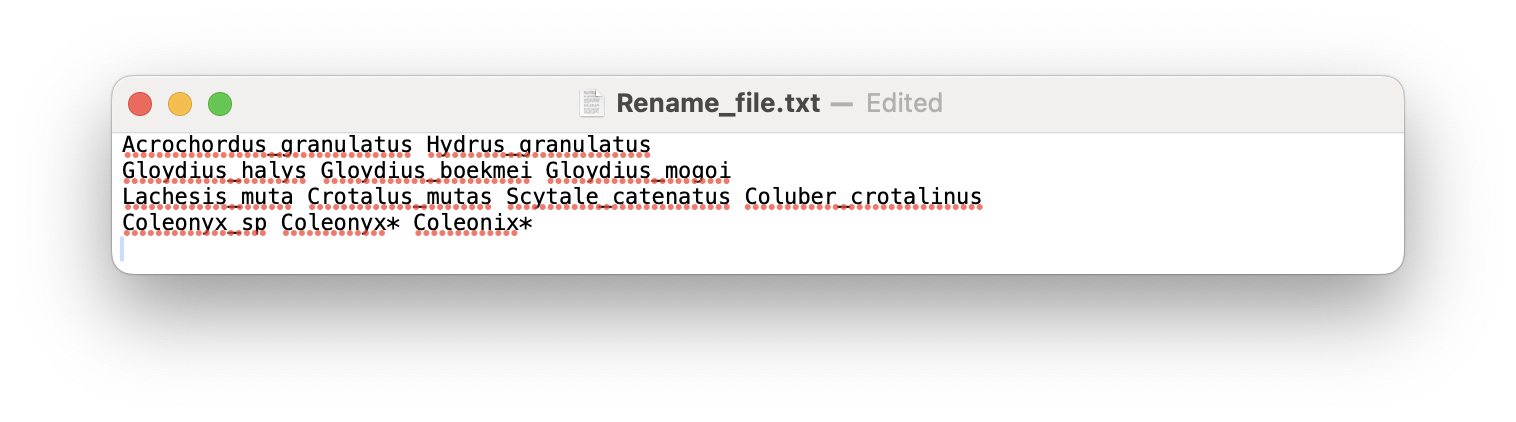
\includegraphics[width=0.8\textwidth]{Rename_file.jpg}
		\caption{Renaming text file containing the lists of terminal taxa to be renamed.}
		\label{renamefile}
		\end{figure}
		}
	\end{phygdescription}
	
	\subsubsection{Arguments}
	
	\begin{description}
	
		\item [STRING list]  The first argument is the ``new name'' for the remainder of the 
		following arguments.
		
	\end{description}
		
	\subsubsection{Defaults}
		None.
		
	\begin{example}
	
		\item{\texttt{rename("a","b","c")}\\ Renames the terminal names ``b'' and ``c'' to 
		the terminal name ``a''.}
		
	\end{example}


%--------------------------------------------------------------------------------------------------------------------------------	
%report
%--------------------------------------------------------------------------------------------------------------------------------				
\subsection{Report}
\label{subsec:report}
	\subsubsection{Syntax}
		\texttt{report([STRING, argument list])}
	
	\begin{phygdescription}
		{Outputs the results of the current analysis to a file or to \texttt{stderr}. To redirect the 
		output to a file, the file name (in quotes), followed by a comma, must be included in 
		the argument list of report. All arguments for \texttt{report} are optional. This command 
		allows the user to output information concerning the characters and terminals, 
		diagnosis, export static homology data, implied alignments, trees, graphs, dot files, 
		as well as other miscellaneous arguments. By default, new information printed to 
		a file is appended to that file. The option \texttt{overwrite} overrides the default and 
		rewrites the file. Many of the report options are output in csv format, which can
		subsequently be imported into spreadsheet programs like \textit{Excel} or 
		\textit{Numbers} for easy viewing.}
	\end{phygdescription}
	
	\subsubsection{Arguments}
	\begin{description}
		
		\item[append] When reporting data or graphs to a file, this information is 
		appended to the end of the file. By default, files are appended to the report, 
		rather than overwritten. Compare with the \texttt{overwrite} argument.

		\item[ascii] Reports ASCII character representations of the reported graphs.
		This information will be directed to a file, in csv format, if a file name (in quotes), 
		followed by a comma, is included in the argument list of report. If no file name is 
		specified, this information will be printed to the stderr. This file can be viewed 
		in any text editor. 
		
		\item[branchlengths] When reporting graphs, \phyg will report the branch 
		lengths of these graphs. In Newick and eNewick files, branch lengths 
		follow the terminal names, separated by a colon. In eps and pdf files, 
		branch lengths appear above the branches. In ASCII and dot files, branch 
		lengths follow the terminal labels. This is the default. Compare with 
		\texttt{nobranchlengths}. 

		\item[collapse] Specifies that zero length branches are collapsed. If a dotpdf 
		graph is specified, the branches are collapsed by default. If ASCII, Newick, 
		eNewick and dot are specified, the zero length branches are not collapsed by 
		default. Compare with the \texttt{nocollapse} argument.  		
		
		\item[crossrefs] Reports whether data are present or absent for each terminal 
		in each of the imported data files. The argument will report a table with terminals 
		represented in rows, and the data files in columns. A plus sign (`+') indicates that 
		data for a given terminal is present in the corresponding file; a minus sign (`--') 
		indicates that it is absent. This provides a comprehensive visual overview of the 
		completeness of the data. It will highlight missing data, as well as inconsistencies 
		in the spelling of taxon names in different data files (see Figure \ref{crossrefs}).  
		This information will be directed to a file, in csv format, if a file name (in quotes), 
		followed by a comma, is included in the argument list of report. If no file name is 
		specified, this information will be printed to the stderr.
		
		\begin{figure}
		\centering
		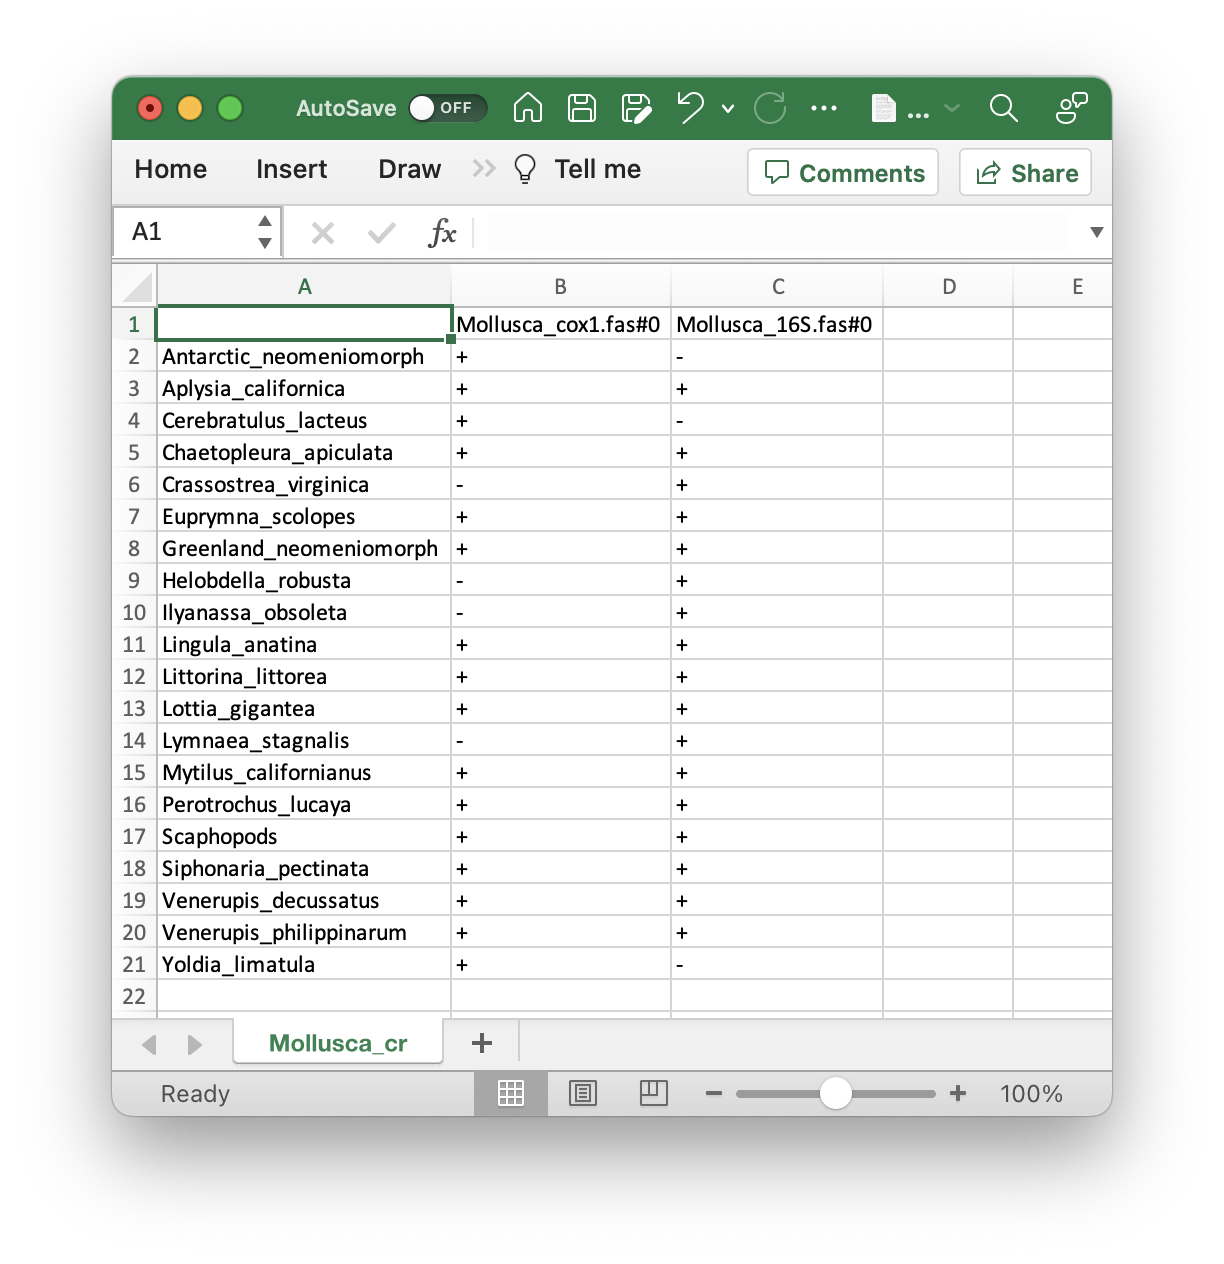
\includegraphics[width=0.55\textwidth]{crossrefs1.png}
		\caption{The figure shows a crossrefs files, which has been imported into 
		\textit{Excel}.}
		\label{crossrefs}
		\end{figure}
			
		\item[data] Outputs a summary of the input data and terminals. Information relating 
		to the input data (number of terminals, number of input files, number of character 
		blocks and the total number of characters) is summariazed. It also provides
		information relating to the terminal taxa included in the analysis, including the 
		names of the taxa, a list of the excluded taxa (if any), and whether any terminals 
		were renamed. In this file you will also see information relating to ``Index'', ``Block'', 
		``Name'', ``Type'', ``Activity'', ``Weight'', ``Prealigned'', ``Alphabet'', and ``TCM''. 
		``Index'' reports the character number in the overall dataset; ``Name'' reports the 
		name of the character (by default based on its source data file); ``Type'' is the type 
		of character (e.g. Non-Additive, Matrix, Nucleotide Sequence), ``Activity'' reports 
		whether the character is active (included in the analysis) or not (excluded), 
		``Weight'' is the weight of the character, ``Prealigned''  denotes whether a 
		sequence character (e.g. amino acids) is to treated as prealigned or not, 
		``Alphabet'' the elements of a sequence character, ``TCM'' is the transition cost 
		matrix specifying costs among sequence elements and ``gap'' or insertion-deletion.
		This information will be directed to a file, in csv format, if a file name (in quotes), 
		followed by a comma, is included in the argument list of report. If no file name is 
		specified, this information will be printed to the stderr.
	
		\item[diagnosis] Outputs graph diagnosis information such as vertex, states 
		and edge statistics. This information will be directed to a file, in csv format, if a 
		file name (in quotes), followed by a comma, is included in the argument list of 
		report. If no file name is specified, this information will be printed to the stderr.
		
		\item[displaytrees] Reports graph information for softwired networks. The 
		`display' trees are output for each data block. This information will be directed 
		to a file, if a file name (in quotes), followed by a comma, is included in the 
		argument list of report. If no file name is specified, this information 
		will be printed to the stderr.
		
		\item[dot] Outputs a graph in dot format. The dot file can be viewed (and 
		modified) in \textit{Graphviz} (see also \texttt{dotpdf}). In order to output pdf 
		files the application \textit{dot} must be installed from the 
		\href{https://graphviz.org/download/}{Graphviz} 	website. Graphviz is 
		open-source graph visualization software. \texttt{dot} is the default graph 
		representation---a dot file will only be reported if no other graph type is specified. 
		
		\item[dotpdf] Outputs two files---a graph file in dot format, along with either
		an eps (on MacOS) or pdf (on Linux) (see also \texttt{dot}). The eps and pdf 
		files can be read in \textit{Adobe Illustrator}, \textit{Apple Preview} or any 
		vectorial image edition program.  By default, when \texttt{dotpdf} is specified,
		edges are collapsed (contracted) if they have a minimum weight (length) of 0.
		
		\item[graphs] Outputs a graph in the format specified by the other arguments 
		in the command. These are either Newick, eNewick, ASCII, dot, and dotpdf, 
		which will output a graph in eps (on MacOS) or pdf (on Linux) format.
		
		\item[htulabels] Labels the HTUs in the output files. This is the default. Compare 
		with \texttt{nohtulabels}.
		
		\item[ia] Synonym of \texttt{impliedalignment}.
		
		\item[impliedalignment] Outputs the implied alignments of the specified 
		set of characters in FASTA or FASTC (depending on sequence type) format. 
		This argument is synonymous with the argument \texttt{ia}. By default, 
		an implied alignment is reported for each block of input data. 
		
		\begin{description}
		
			\item[concatenate] This optional argument can be used with \texttt{ia}
			| \texttt{impliedalignment}. Instead of outputting an implied alignment 
			for each block of input data, it will report a file with all the implied 
			alignments concatenated into a single file.
			
			\item[includemissing] Outputs a FASTA or FASTC (depending on sequence type), 
			including taxa that are missing data for that particular block of data in the implied 
			alignment.
			In this case, \phyg will print question mark characters (`?') for the missing taxon in 
			this block of the implied alignment. This option interacts nicely with 
			\texttt{concatenate} in creating prealigned FASTA (implied alignments) 
			with all the terminals included for all the data. By default, taxa with 
			missing data are not included.
			
		\end{description}
				
		\item[newick] Outputs graphs in the eNewick or Newick format, with the terminals
		separated with commas, and graphs separated with semicolons. Branch
		lengths follow terminals, separated by a colon.
		
		\item[nobranchlengths] When reporting graphs, \phyg will by default 
		report the branch lengths of these graphs. In Newick and eNewick files, 
		branch lengths follow the terminal names, separated by a colon. In eps 
		and pdf files, branch lengths appear above the branches. In ASCII and 
		dot files, branch lengths follow the terminal labels. The argument
		\texttt{nobranchlengths} will override this default and branch lengths 
		of graphs are not reported.
		
		\item[nocollapse] Specifies that zero length branches are not collapsed.
		If ASCII, Newick, eNewick and dot graphs are specified, the zero length 
		branches are not collapsed by default. In contrast, if a dotpdf graph is 
		specified, the zero-length branches are collapsed. Note: by specifying 
		a dotpdf file, this will by default also output a dot file---in both these files 
		zero length branches are collapsed. Compare with the \texttt{collapse} 
		argument. 
				
		\item[nohtulabels] Labels of the HTUs are not included in the output files. 
		This option can not be applied to eNewick graph. Compare with the argument 
		\texttt{htulabels}.
		
		\item[overwrite] By default, when reporting data or graphs to a file, the 
		information is appended to the end of the file (see \texttt{append}). The 
		option \texttt{overwrite} overrides this default and rewrites the file rather 
		than appending to the existing information.

		\item[pairdist] Outputs a taxon pairwise distance matrix in csv format. 
		This information will be directed to a file, if a file name (in quotes), followed 
		by a comma, is included in the argument list of report. If no file name is 
		specified, this information will be printed to the stderr.
		
		\item[reconcile] Outputs a single `reconciled' graph from all graphs in 
		memory. The methods include consensus, supertree, and other supergraph 
		methods as described in \cite{Wheeler2012, Wheeler2022}. When \texttt{reconcile} 
		is specified as a command option a series of other options may be specified 
		to tailor the desired outputs:
		
		\begin{description}
		
			\item [Compare:] Specifies how group comparisons are to be made.
						
			\begin{description}
				\item[combinable] Group comparison are made by identical match 
				[(A,(B,C))$\neq$(A,B,C)]. This is the default.	
								
				\item[identity] Group comparison are made by combinable components sensu 
				     \cite{Nelson1979} [(A,(B,C)) consistent with (A,B,C)]. This option can be used 
				     to specify `semi-strict' consensus \citep{Bremer1990}.
				     
			\end{description}
			
			\item [Connect:BOOL] Specifies that the output graph be connected 
			(single component), potentially creating a root node and new edges labeled 
			with ``0.0''. The default value is TRUE. This option will connect any forest elements
			into a single graph. 
			
			\item [Method:] Specifies the reconciliation method when more than a single
			   graph is returned.
			
			\begin{description}
			
				\item[Adams] Specifies that returned graphs should be reconciled using the 
				Adams II consensus \citep{Adams1972} method.
				
				\item[cun] Graphs are reconciled using the Cluster Union Network 
				\citep{Baroni2005} method. This argument can be used in conjunction with 
				\texttt{threshold}. 
				
				\item[eun] Graphs are reconciled using the Edge-Union-Network method of 
				\citep{MiyagiandWheeler2019}. This argument can be used in conjunction with 
				\texttt{threshold}. This is the default.
				
				\item[majority] Specifies that values between 0 and 100 of either vertices or 
				edges will be retained. If all inputs are graphs with the same leaf set this will 
				be the Majority-Rule Consensus \citep{MargushandMcMorris1981}. This
				argument is used in conjunction with \texttt{threshold}.

				\item[strict] This option requires all vertices are present to be included in the final 
				graph. If all inputs are graphs with the same leaf set this will be the Strict Consensus 
				\citep{Schuhandpolhemus1980}. 
				
				\item [Threshold:INT] Specifies the threshold frequency (between 0 and 100) 
				of vertex or edge occurrence in input graphs to be included in the output graph. 
				This value affects the behavior of `eun', `cun', and `majority'. The 
				default value is $0$.
				
			\end{description}
		
			\item [EdgeLabel:BOOL] Specifies the output graph have edges 
			labeled with their frequency in input graphs. The default value is TRUE.			
			
			\item [VertexLabel:BOOL] Specifies the output graph have vertices 
			labeled with their subtree leaf set. The default value is FALSE.	
				
		\end{description}	
				
		\item[search] Outputs search statistics in csv format. See Section 
		\ref{subsec:search} for details about the randomized series of graph 
		optimization methods included in each iteration of a timed search.
			
		\item [STRING] Specifies the name of the file to which all types of report 
		outputs, designated by additional arguments, are printed. If no additional 
		arguments are specified, a graph in dot format, along with an eps or pdf 
		file (depending on the operating system) will be reported to a file named 
		`\textbf{defaultGraph}'. By default, files are appended to the report, rather 
		than overwritten (see \texttt{overwrite}).
				
		\item[support] Outputs support graphs (see Section \ref{subsec:support})
		that have been previously calculated by the command \texttt{support}. 
		Resampling graphs \citep{Farrisetal1996} are independent of the input graphs 
		while Goodman-Bremer graphs \citep{Goodmanetal1982, bremer1994} are 
		based on current graphs. Graphs can be output in multiple formats with the
		use of the options \texttt{ascii}, \texttt{newick}, \texttt{enewick}, \texttt{dot}, 
		and depending on your operating system, \texttt{dotpdf} for pdf (Linux) or 
		eps (MacOS). See Section \ref{sec:outputgraphs} for information relating to 
		viewing and installation requirements. Should you fail to choose one of 
		these reporting formats, \phyg will issue a warning in the output display 
		of the \textit{Terminal} window, and output a `dot' file that can be processed 
		later.
		
		\item[tnt] Outputs information in TNT \citep{Goloboffetal2008} format (see 
		Section \ref{subsec:TNT}) using \texttt{impliedAlignment} for unaligned 
		sequences. This information will be directed to a file, in csv format, if a file 
		name (in quotes), followed by a comma, is included in the argument list of 
		report. If no file name is specified, this information will be printed to the stderr.
				 
	\end{description}			
		
	\subsubsection{Defaults}
		\texttt{report(append, branchlengths, collapse, dot, htulabels)}
		The default graph representation is \texttt{dot}. A dot file will only be 
		reported if no other graph type is indicated. Branch lengths and HTU 
		labels are printed in the output files. Zero length branches are collapsed. 
		When writing to a file, the information is appended to the end of the file. 
		
	\begin{example}
	
		\item{\texttt{report("outFile.tre", newick, overwrite)}\\ Outputs graphs in newick 
		format to the file ``\textbf{outFile.tre}'', overwriting any existing information.
		In addition, zero length branches are collapses and branch lengths and HTU 
		labels are printed in the output files (the default).}
		
		\item{\texttt{report("outFile\_cr.csv", crossrefs)}\\ Outputs the cross reference file 
		``\textbf{outFile\_cr.csv}'' with data pertaining to the presence and absence of 
		taxa in the input files. This information is appended to the end of the file (the 
		default), if existing information exists.}
		
		\item{\texttt{report("outFile", dot, reconcile, method:eun, threshold:51)}\\ Outputs a
		graph which has been reconciled using the Edge-Union-Network method with a 
		minimum edge frequency of 51\%. The graph is outputted in dot format to the 
		file ``\textbf{outFile}', appending to any existing information in the file.}
		
		\item{\texttt{report("outFile\_supports", support, dotpdf)}\\ Outputs a graph file in 
		dot format, along with either an eps (on MacOS) or pdf (on Linux) (see also dot). 
		Support values appear above branches in the eps or pdf graphs, and are \hl{...}.
		Support values are generated in the script using the command \texttt{support}
		will appear above the branch in the eps or pdf files.}
		
	\end{example}
		
%---------------------------------------------
%run
%---------------------------------------------		
\subsection{Run}
	\subsubsection{Syntax}
		\texttt{run(STRING)}
		
	\begin{phygdescription}
		{Executes \phyg script file(s) containing commands. The filename must be 
		included in quotes. Executing scripts using \texttt{run} can be useful to specify 
		common actions such as inputting file(s) and graph construction.}
	\end{phygdescription}
	
	\subsubsection{Arguments}
	\begin{description} 
		
		\item[STRING] The only argument is the name of the script-containing file
		 containing the commands to be executed.
		 
	\end{description}
		
	\subsubsection{Defaults}
		There are no default settings of \texttt{run}. 
	
	\begin{example}
	
		\item{\texttt{run("readFiles.pg")}\\ Executes ``\textbf{readFiles.pg}'', which 
		may contain multiple input files to be \texttt{read}.}
		
		\item{\texttt{run("searchCommands.pg")}\\ Executes ``\textbf{searchCommands.pg}'', 
		which may contain commands defining a common search strategy (e.g. 
		\texttt{build}).}
		
	\end{example}

%---------------------------------------------
%search
%---------------------------------------------		
\subsection{Search}
\label{subsec:search}
	\subsubsection{Syntax}
		\texttt{search([argument list])}
	
	\begin{phygdescription}
		{This command implements a randomized search strategy, performing a timed 
		 series of graph optimization methods including building, swapping, 
		recombination (fusing), simulated annealing and drifting, network edge edits
		(addition, deletion and moving), and Genetic Algorithm. The parameters and 
		their order of implementation are randomized. The arguments 
		associated with this command specify the duration and number of independent 
		instances of the \texttt{search}. Successive rounds of \texttt{search} gather any 
		solutions from previous sequential or parallel rounds, as well as any input graphs. 
		Since search methods may vary in how long they take, individual iterations may 
		take longer than the specified duration.  By default, search strategies are chosen 
		uniformly at random, and if \texttt{Thompson} is specified, Thompson sampling 
		\cite{Thompson1933,WheelerThompson} is used to modify the probabilities 
		of search strategies over the search duration.
		
		When performing a \texttt{search} it is important to set the maximum amount of time, 
		such that the program has a reasonable amount of time to complete the search. 
		Therefore, it is important to have some idea as to the length of time it would take 
		to do a single round of searching. Performing a simple search that includes 
		build, swap, and network edits (if applicable) and calculating the amount of time 
		for a single graph within this search provides some approximation as to the amount 
		of time necessary to perform a thorough search. Obviously, this estimate is data and 
		optimality criterion dependent. With this information, the user can then estimate the 
		amount of time necessary to perform a thorough search (perhaps 10 times the 
		amount of time it took to perform this simple search). It is recommended to perform 
		a \texttt{swap(joinAll)} (see Section \ref{subsec:swap}) after the \texttt{search} has 
		completed. The user should also allow some time for the program to collate and 
		write the results to files.}
	\end{phygdescription}
			
	\subsubsection{Arguments}
	\begin{description}
	
		\item[days:INT] Adds the number of days (as specified by the integer) to the 
		maximum total execution time for the search.
		
		\item[hours:INT] Adds the number of hours (as specified by the integer) to the 
		maximum total execution time for the search.
		
		\item[instances:INT] Specifies the number of (potentially parallel) simultaneous
		searches (instances), as indicated by the integer value. The overall search will 
		terminate only when all instances have completed.
		
		\item[maxNetEdges:INT] Limits the maximum number of network edges to that
		specified by the integer value. This should only to be used if \texttt{graphtype}
		has been \texttt{set} to \texttt{hardwired} or \texttt{softwired}. 
		
		\item[minutes:INT] Adds the number of minutes (as specified by the integer) to 
		the maximum total execution time for the search.
		
%		\item[simple] Only internal---used for testing purposes.
		
%		\item[seconds:INT] Adds the number of seconds (as specified by the integer) to the 
%		maximum total execution time for the search. Only internal---used for testing purposes.

		\item[stop:INT] Causes a search instance to terminate after the number of iterations 
		without graph optimality improvement. This argument is an adjunct to the specified 
		time. The search iteration will continue until the maximum execution time for the search 
		has ended or until the cost of the best graph fails to improve after the specified integer 
		(whichever comes first). The overall search will terminate only when all instances have 
		completed.
		
		\item[Thompson:INT] Specifies that the randomized choice of search option (e.g. 
		Wagner Build, SPR, Genetic Algorithm) employs Thompson sampling \citep{Thompson1933}. 
		This form of sampling uses machine learning techniques to guide the randomized option 
		selection of the search \citep{WheelerThompson}. This sampling method is a heuristic for 
		timed search decision making. The integer value specifies the memory value for the Thompson 
		sampling. The lower the value (down to 0), the shorter the memory allowing for more rapid 
		adjustment of search strategy probabilities. This parameter is applied to both the \texttt{linear} 
		and \texttt{exponential} arguments of \texttt{Thompson}.
			
		\begin{description}
		
			\item[exponential] Specifies that the Thompson memory is an exponential function of 
			$m$ (the \texttt{INT} value specified by \texttt{Thompson} above). Updating of search 
			type, $\theta^k$, probability for iteration $n$ is $ \left(1 - \frac{1}{2^m} \theta^k_{n-1}\right) 
			+ \left(\frac{1}{2^m} \theta^k_n \right)$. Thompson success is a function of whether a 
			search was successful in reducing the graph cost and how long that search took to 
			complete.
			
			\item[linear] Specifies that the Thompson memory is a linear function of $m$ (the 
			\texttt{INT} value specified by \texttt{Thompson} above). Updating of search type, $\theta^k$, 
			probability for iteration $n$ is $\frac{m}{m+1} \theta^k_{n-1} + \frac{1}{m+1} \theta^k_n$.  
			Thompson success is a function of whether a search was successful in reducing the graph 
			cost and how long that search took to complete.

		\end{description}
		
	\end{description}		
	
	\subsubsection{Defaults}
		\texttt{search(instances:1, seconds:30)} Under the default parameters, \phyg will perform 1 
		instance of a search for at most 30 seconds.
		
	\begin{example}
	
		\item{\texttt{search(hours:10, instances:2)}\\ Performs 2 searches (instances) for 10 hours 
		each. These searches will be performed simultaneously if the computer capacity allows.}
				
		\item{\texttt{search(hours:10, minutes:30)}\\ Performs a single search instance (the default) 
		for 10 hours and 30 minutes.}
		
		\item{\texttt{search(days:1, thompson:2, linear)}\\ Employs Thompson sampling to guide the 
		randomized option selection of the search. The Thompson memory value is a linear function 
		of the parameter 2. This search is performed for 1 day.}
		
	\end{example}
	
%---------------------------------------------------------------------------------------------------------------------------------
%select
%---------------------------------------------------------------------------------------------------------------------------------		
\subsection{Select}
	\subsubsection{Syntax}
		\texttt{select([argument list])}
	
	\begin{phygdescription}
		{Specifies the method for choosing and number of graphs to be saved at any point 
		during the analysis. When multiple graphs are present, the \texttt{select} command 
		will specify which graphs are retained for subsequent analysis or reporting.}
	\end{phygdescription}
				
	\subsubsection{Arguments}
	\begin{description}
		
		\item[all] Specifies all the graphs are kept.
		
		\item[atRandom:[INT]] Randomly selects the graphs irrespective of cost. The 
		number of chosen graphs can be specified with an integer value. This can 
		be a useful tool for randomized searches and subsequent analyses where 
		randomized sampling is desired.
			
		\item[best:[INT]] Selects the number of best or lowest cost graphs. The number 
		of returned graphs can be specified by the integer value. If no integer value is 
		specified, all of the graphs of best optimality value will be returned. If the number 
		of optimal graphs exceeds the value of best, the subset of optimal graphs are 
		chosen in an undefined but consistent order.
							
		\item[threshold:FLOAT] Keeps all the best (shortest) graphs and all the unique 
		graphs up to the fraction longer than shortest graph. This fraction is specified by 
		the \texttt{FLOAT}.
			
		\item[unique:[INT]] Selects only topologically unique graphs, irrespective of their
		cost. The program will keep as many graphs as specified by the integer value.
			
	\end{description}

	\subsubsection{Defaults}
		\texttt{select(best)} Keeps all unique graphs of best optimality value.
		
	\begin{example}
	
		\item{\texttt{select(atrandom:10)}\\ Keeps up to 10 graphs, selecting the graphs
		 at random.}
						
		\item{\texttt{select(best:10)}\\ Keeps up to 10 graphs of best optimality value.}
		
		\item{\texttt{select(threshold:0.5)}\\ Keeps all the graphs of best optimality value
		and the unique graphs that are up to 50\% longer than these graphs.}
		
	\end{example}

%--------------------------------------------------------------------------------------------------------------------------------
%set
%--------------------------------------------------------------------------------------------------------------------------------				
\subsection{Set}
\label{subsec:set}
	\subsubsection{Syntax}
		\texttt{set(argument string)}
	
	\begin{phygdescription}
		{Changes the settings of \texttt{PhyG}. This command performs an array of functions
		from specifying the seed of the random number generator, to selecting a terminal for
		rooting output graphs, to specifying  graph type, final assignment, and optimality 
		criterion. All \texttt{set} commands are executed at the start of a run, irrespective of
		where they appear in the script. The command \texttt{transform} is used to modify 
		global settings during a run (see \texttt{transform} Section \ref{subsec:transform}).
		\texttt{set} arguments have to be indicated on separate lines of the script, otherwise
		\phyg will return an error.}
	\end{phygdescription}
			
	\subsubsection{Arguments}
	\begin{description}
		
%		\item[bc2] Related to Information Theory. Not implemented yet.
		
%		\item[bc4] Related to Information Theory. Not implemented yet.
	
%		\item[bc5] Related to Information Theory. Not implemented yet.
		
%		\item[bc8] Related to Information Theory. Not implemented yet.
		
%		\item[bc64] Related to Information Theory. Not implemented yet.
		
%		\item[bcgt64] Related to Information Theory. Not implemented yet.
		
%		\item[compressResolutions:True|False] 
%		Determines whether softwired graph resolutions are ``compressed'' if multiple 
%		vertex assignments in alternate display trees are equal in subtree leaf set, only 
%		the first lowest cost resolution is retained. This option can significantly reduce 
%		the time to evaluate softwired graphs, but can increase the optimality score of 
%		the graph. This can be used in combination with \texttt{transform(compressResolutions:True)} 
%		or \texttt{transform(softwiredMethod:\\Exhaustive)} 
%		at a later stage to improve graph score. Not implemented yet.
			
		\item[criterion:] Sets the optimality criterion for graph search.
			
		\begin{description}
			
			\item[parsimony] Graph costs are determined by the parsimony criterion, 
			that is the minimum sum of transformation events multiplied by their weights. 
			This is the default.
			
			\item[ncm] Graph costs are determined by the No-Common-Mechanism 
			likelihood model of \citep{TuffleyandSteel1997}. This is exact for trees, but 
			for networks should be treated as a form of character weighting.  
			
		\end{description}
			
%		\item[defparstrat] Only internal---used for testing purposes.

		\item[dynamicepsilon:[FLOAT]] Alters the performance of the heuristic graph cost 
		calculations to force a full graph evaluation more frequently. This will slow down the
		search but has the potential to identify better solutions. The float indicates the additional 
		cost factor in evaluating the graphs.
			
		\item[finalAssignment:] Sets the method of determining the `final' sequence states. 
						
		\begin{description}
			
			\item[DirectOptimization] DirectOptimization uses the DO method to assign 
			the final states. This is more time consuming than \texttt{ImpliedAlignment}. 
			DO has an additional factor of potentially $O(n^2)$ in sequence length compared 
			to the constant factor for IA due to additional graph traversals. This is the default.

			\item[DO] Synonym of \texttt{DirectOptimization}.
			
			\item[IA] Synonym of \texttt{ImpliedAlignment}.
			
			\item[ImpliedAlignment] Uses implied alignments to assign the final states. This 
			final assignment procedure has a lower time complexity than DO.
			
		\end{description}
			
		\item[graphFactor:] Sets the network penalty for a softwired network. When conducting 
		a network analysis, a penalty can be specified, so that ‘softwired’ phylogenetic networks 
		can compete equally with phylogenetic trees on a parsimony optimality basis. A network 
		penalty takes into account the change in cost as edges are added to the graph. Hardwired 
		graphs are automatically set to \texttt{NoPenalty}.
			
		\begin{description}
			
			\item[nopenalty] No penalty is added.	

			\item[w15] Employs the parsimony network penalty of \cite{Wheeler2015}.	
		
			\item[w23] Sets the parsimony network penalty of \cite{WheelerandWashburn2023}, 
			which is more severe (the penalty is applied to all the blocks) but has a lower time 
			complexity than W15.		

		\end{description}
			
		\item[graphsSteepest:[INT]] Sets the maximum number of graphs to be evaluated 
		simultaneously during `steepest' descent in swapping and network addition and 
		deletion operation. The number is the lower of the number of parallel threads 
		and $n$ (default 10).  Setting this number to higher values can improve the use of 
		parallel resources, but at the cost of additional memory footprint. Accordingly, 
		reduction in this value can reduce memory consumption.
			
		\item[graphType:] Sets the phylogenetic graph type. The program allows for the input, 
		analysis of and output of a broad class of phylogenetic graphs. These include trees, 
		and both `softwired’ and `hardwired’ networks. 
			
		\begin{description}
			
			\item[tree] Sets the graph type to tree. This is the default.
		
			\item[hardwired]  Sets the graph type to hardwired. A `hardwired' network is 
			one where characters can have multiple parents.
	
			\item[softwired]  Sets the graph type to softwired. A `softwired' network is 
			a summary of a set of individual `display' trees that have been generated by 
			removing edges from the network. Individual characters have single parents.	
						
		\end{description}
			
%		\item[jointhreshold] Only internal---used for testing purposes.

%		\item[lazyparstrat] Only internal---used for testing purposes.

		\item[missingThreshold:[INT]] Sets the maximum percentage of missing data in a 
		terminal. The default setting is 100, leaving all terminals in the data set. Terminal taxa
		with more than the missing fraction are deleted.  The \texttt{missingThreshold} value is 
		determined by the number of input blocks (files). Hence, a taxon with all missing values 
		in a TNT file will be counted as not missing for this purpose.   
		
%		\item[modelcomplexity] Related to Information Theory. Not implemented yet.
		
		\item[multiTraverse:[BOOL]] Controls the multi-traverse character optimization 
		option. If \texttt{True}, character trees are traversed from each edge as in 
		\citep{VaronandWheeler2012,VaronandWheeler2013, POY4, POY5}, but 
		individually for each dynamic character. This is the default and yields better 
		(lower) optimality scores at the cost of added execution time. This is the default.
		If \texttt{False}, only outgroup-based traversals are performed as in 
		\citep{Wheeler1996, POY2, POY3}. 
					
		\item[outgroup:STRING] Specifies the terminal to root the output trees. 
		This name must appear in double quotes. If the outgroup is not set, the 
		default outgroup is the taxon whose name is lexically first after any renaming 
		of taxa, and/or if taxa were specified by using the arguments \texttt{include} 
		or \texttt{exclude}. Only a single taxon can be set as the outgroup of the analysis. 
					
		\item[partitioncharacter:STRING] Sets the character that is used to partition the 
		data. Sequences can be divided into smaller fragments using an assigned character. 
		This single character is chosen by the user (unlike in POY, where the pound sign 
		(`\textbf{\#}') was the only option to partition datasets). Each fragment is treated as an 
		individual character. When partitioning the data in this way, the number of partitions 
		must be the same across homologous sequences. The default is `\textbf{\#}'.

%		\item[reportnaive] Only internal---used for testing purposes.

		\item[rootCost:] Sets the root cost for a graph. 	
				
		\begin{description}
			
			\item[noRootCost]  No cost is ascribed to the root. This is the default for parsimony searches.
			
			\item[w15] Sets a cost at $\frac{1}{2}$ the cost of `inserting' the root character 
			assignments. The W15 root cost is based on the same rationale as the parsimony 
			network penalty of  \cite{Wheeler2015}.

		\end{description}
			 
		 \item[seed:INT] Sets the seed for the random number generator using the integer
		 value. If unspecified, \phyg uses the system time as the seed. By setting this value, 
		 we are guaranteed to reproduce a given search trajectory each time the script is run. 
		 This is the case even when the operations are randomized, as is the case when using 
		 the argument \texttt{atrandom}.
			 
		 \item[softwiredMethod:] Sets the algorithm for softwired graphs to the 
		 `Naive' method of diagnosing all display trees, as in \cite{Wheeler2015} or
		 the `Resolution Cache' method of \cite{WheelerandWashburn2023}.
		 
		\begin{description}
			
			\item[Naive] Determines the score of a softwired network by evaluating all display 
			trees (up to $2^m$ for $m$ network nodes) and summing the costs of the minimum 
			cost display tree for each block of data. This can be extremely time consuming for 
			graphs with large number of network nodes.
			
			\item[ResolutionCache] Uses the method of \citep{WheelerandWashburn2023} to 
			determine softwired network costs in greatly reduced time.  This is the default.
			
		\end{description}
		
%		\item[strictparstrat] Only internal---used for testing purposes.

		\item[useia] Uses implied alignments to do as many of the calculations as possible.
		This method is faster, but approximate. 
		
		\item[usenetaddheuristic]	Uses heuristic graph cost calculations when adding network
		edges to the graph.
		
	\end{description}
					
	\subsubsection{Defaults} 
		\texttt{set(criterion:parsimony)}\\
		\texttt{set(FinalAssignment:DirectOptimization)} \\
		\texttt{set(graphFactor:w15)} \\
		\texttt{set(graphtype:tree)}\\
		\texttt{set(outgroup:STRING)} The default outgroup is the taxon whose name is 
		lexically first after renaming of taxa and/or if taxon were specified for inclusion or
		exclusion. 
		
%		\texttt{CompressResolutions} 
%		is set to \texttt{True}, 
%		and \texttt{PMDL} if PMDL is set as the optimality criterion. The default rootCost
%		is \texttt{noRootCost} if parsimony is the optimality criterion and \texttt{PMDL} if PMDL is set 
%		as the optimality criterion.
		
	\begin{example}
	
		\item{\texttt{set(criterion:parsimony)}\\Sets the graph search optimality criterion to 
		parsimony.}

		\item{\texttt{set(outgroup:"Lingula\_anatina")}\\This command selects the terminal 
		"Lingula\_anatina" and sets it as the outgroup for the analysis.}
		
		\item{\texttt{set(partitioncharacter:@)}\\Sets the partition character in the input dataset 
		to the at sign `@'.}
		
%		\item{\texttt{set(compressResolutions:False)}\\Turns off softwired graph resolution compression.}

	\end{example}

%--------------------------------------------------------------------------------------------------------------------------------
%support
%--------------------------------------------------------------------------------------------------------------------------------			
\subsection{Support}
\label{subsec:support}
	\subsubsection{Syntax}
		\texttt{support([argument list])}
		
	\begin{phygdescription}
		{Generates graph supports via resampling \citep{Farrisetal1996} and Goodman-Bremer  
		\citep{Goodmanetal1982, bremer1994}. Currently, Jackknifing, Bootstrapping and 
		Goodman-Bremer supports are the resampling methods that are implemented. If
		the criterion is set to \texttt{ncm} (see Section \ref{subsec:set}), the support values 
		for Goodman-Bremer are log likelihood ratios.}
	\end{phygdescription}
		
	\subsubsection{Arguments}
		\begin{description}
		
%		\item[atRandom] When testing support for network edges, it randomizes the evaluation.
%		Only internal---used for testing purposes.

		\item[bootstrap] Calculates Bootstrap support. The user can specify the number of 
		iterations, using \texttt{replicates}. The edges are labeled with the bootstrap 
		frequencies when output via the command \texttt{report(support)}. Default replicate 
		search is 100 random addition sequence distance-based Wagner builds and TBR 
		branch swapping on the best distance tree. If the graph type is softwired or hardwired, 
		\texttt{netadd}, \texttt{maxnetedges:5}, \texttt{atrandom} are added. 
		
		\item[buildonly] Performs very rapid, but not extensive graph searches for each 
		resampling replicate.
		
		\item[gb] Synonym of GoodmanBremer.
			
		\item[goodmanBremer] Specifies that Goodman-Bremer support is 
		calculated for input graphs. 
			
		\begin{description}
			
			\item[gbsample:[INT]] Specifies the number of alternate graphs to be examined 
			(i.e. limited). The graphs are chosen uniformly at random.  This is used to reduce 
			execution time of the Goodman-Bremer support at a cost of potentially increased 
			overestimates (higher upper bound values). 
			
			\item[spr] Traverses the SPR neighborhood to determine an upper-bound on 
			the NP-hard values.
			
			\item[tbr] Traverses the TBR neighborhood 
			as optionally specified (TBR as default) to determine an upper bound on the NP-hard 
			values (this is the method used in POY v2; \citealp{POY2} \textit{et seq.}).
			
		\end{description}
		
		\item[jackknife:[FLOAT]] Specifies that Jackknife resampling is performed with $n$ 
		acceptance probability (default 0.6231 or $1 - e^{-1}$). When reported (via 
		\texttt{report(support)}), edges are labeled with the jackknife frequencies. Default 
		replicate search is 100 random addition sequence distance-based Wagner builds 
		and TBR branch swapping on the best distance tree. If the graph type is softwired 
		or hardwired, \texttt{netadd}, \texttt{maxnetedges:5}, \texttt{atrandom} are added. 
		
		\item[replicates:[INT]] Specifies the number of resampling replicates, as indicated by the 
		integer value, that are performed in resampling support for Jackknife and bootstrap methods. 
		The default is 100.
		
	\end{description}	
		
	\subsubsection{Defaults}
		\texttt{support(goodmanBremer:TBR)} Calculates Goodman Bremer support values, 
		via traversing the TBR neighborhood.
		
		\begin{example}
		
			\item{\texttt{support(jackknife:0.50, replicates:1000)}\\Performs 1000 replicates of 
			delete 50\% jackknife resampling.}
				
			\item{\texttt{support(gb, SPR, gbSample:10000)}\\Produces Goodman-Bremer 
			support based on $10,000$ samples of the SPR neighborhood.}
			
		\end{example}

%--------------------------------------------------------------------------------------------------------------------------------
%swap
%--------------------------------------------------------------------------------------------------------------------------------		
\subsection{Swap} 
\label{subsec:swap}
	\subsubsection{Syntax}
		\texttt{swap([argument list])}
			
	\begin{phygdescription}
		{Performs branch-swapping rearrangement on graphs. This command implements a 
		group of algorithms referred to as branch swapping, that proceed by clipping
		parts of the given tree and attaching them in different positions. These algorithms 
		include `NNI' \citep{CaminandSokal1965, Robinson1971}, `SPR' \citep{Dayhoff1969}, 
		and `TBR' \citep{Farris1988, swofford1990a} refinement.  Default swapping trajectories 
		are randomized.}
	\end{phygdescription}
		
	\subsubsection{Arguments}
	\begin{description}
	
		\item[all] Turns off all preference strategies to break and join graphs, simply trying all 
		possible rearrangements. The refinement examines the entire rearrangement neighborhood 
		of the current graph before retaining the best (lowest cost) solutions. The user is advised to
		only use this option on small datasets as it can be computationally intensive (and 
		time consuming).

		\item[alternate] Specifies that alternating rounds of \texttt{spr} \citep{Dayhoff1969} 
		and \texttt{tbr} \citep{Farris1988, swofford1990a} refinement are performed.
		
		\item[annealing[:INT]] Specifies the number of rounds of simulated annealing 
		\citep{Metropolisetal1953,Kirkpatricketal1983,Cerny1985} optimization to be performed, 
		as indicated by the integer value (the default is 1). The acceptance of candidate graphs 
		is determined by the probability $e ^ {- (c_c - c_b)/ (c_b * (k_{max} -k)/ k_{max})}$, 
		where $c_c$ is the cost of the candidate graph, $c_b$ is the cost of the current best 
		graph, $k$ is the step number, and $k_{max}$ is the maximum number of steps (set 
		by the argument \texttt{steps}, with a default of 10).
		
		\begin{description}
			
			\item[steps:[INT]] Specifies the number of temperature steps to be performed during 
			simulated annealing (as specified by the \texttt{annealing}) option. The default is 10.
			
		\end{description}
		
		\item[atRandom] Swap neighborhoods are traversed in a randomized order (compare 
		with \texttt{inorder}). 	This will result in different trajectories of the swap space being 
		explored. This is the default.
		
		\item[drift[:INT]] Specifies the number of rounds of the `drifting' form of simulated 
		annealing \citep{goloboff1999} optimization that are performed, as indicated by the integer 
		value (default 1). The acceptance of candidate graphs is determined by the options 
		\texttt{acceptEqual} and \texttt{acceptWorse}. \texttt{drift} differs from \texttt{annealing} 
		in that there are no cooling steps to modify acceptance probabilities. The maximum 
		number of graph changes is set by \texttt{maxChanges}.
			
		\begin{description}
			
			\item[acceptEqual[:FLOAT]] Specifies that equal cost graphs are accepted with the
			probability as set by the FLOAT value. 
			
			\item[acceptWorse[:FLOAT]] The acceptance of candidate graphs is determined by the 
			probability $1/ (wf + c_c - c_b)$, where $c_c$ is the cost of the candidate graph, $c_b$ 
			is the cost of the current best graph, and $wf$ is the values as specified by the float 
			(default 1.0). 	
			
			\item[maxChanges:INT] Specifies that drifting graph changes are limited to the 
			value as specified by the integer (default 15).
			
		\end{description}
		
		\item[ia] Specifies that Implied Alignment \citep{Wheeler2003} assignment are used for 
		branch swapping as opposed to full Direct Optimization for dynamic characters when the 
		graph type is \texttt{tree}.
		
		\item[inOrder] Contra \texttt{atRandom}, swap neighborhoods are always traversed 
		in the same undefined, but consistent order.
		
		\item[joinAll] Turns off all preference strategies to make a join, simply trying all possible 
		join positions for each pair of clades generated after a break. 

%		\item[joinPruned] Only internal---used for testing purposes.
		
%		\item[joinAlternate] Only internal---used for testing purposes.
				
		\item[keep:INT] Specifies the number of equally costly graphs to be retained, as
		determined by the integer value.		
		
		\item[nni] Specifies that NNI refinement \citep{CaminandSokal1965, Robinson1971} 
		is performed.
		
		\item[replicates:[INT]] Sets the number of randomized swap replicate trajectories. 
		Default 1.
		
%		\item[returnMutated] Only internal---used for testing purposes.
		
		\item[spr:[INT]] Specifies that SPR refinement \citep{Dayhoff1969} is performed. If an 
		integer value is specified, the re-addition of pruned graphs will be within $INT$ 
		edges of its original placement.
		
		\item[steepest] Specifies that refinement follows a greedy path, abandoning the 
		neighborhood of the current graph when a better (lower cost) graph is found.  		
		
		\item[tbr:[INT]] Specifies that TBR refinement \citep{Farris1988, swofford1990a} 
		is performed. If an integer value is specified, the re-addition of pruned graphs 
		will be within $2 * INT$ edges of its original placement.
		
	\end{description}	
		
		\subsubsection{Defaults}
			\texttt{swap(alternate, keep:10, steepest)}
		
		\begin{example}
		
			\item{\texttt{swap(tbr, all, keep:10)}\\Performs tbr branch swapping on each current graph 
			returning up to 10 best graphs after examining all graphs in 
			the rearrangement neighborhood.}
			
			\item{\texttt{swap(annealing:10, steps:10)}\\Performs alternating rounds of \texttt{spr} and 
			\texttt{tbr} branch swapping (the default) on each current graph, specifying 10 rounds of
			simulated annealing, with 10 temperature steps being performed for each
			simulated annealing round (the default number of steps).}
			
		\end{example}
	
%--------------------------------------------------------------------------------------------------------------------------------
%transform
%--------------------------------------------------------------------------------------------------------------------------------		
\subsection{Transform}
\label{subsec:transform}
	\subsubsection{Syntax}
		\texttt{transform(argument list)}
			
	\begin{phygdescription}
		{Transforms the properties of the imported characters, graphs, or general values 
		from one value or type to another. It 
		modifies the global settings during program execution (as opposed to \texttt{set}, 
		which operates at the start of the analysis). This includes changes of graph type
		(e.g. tree to softwired Network) and data types (e.g. dynamic to static 
		approximation), among other operations.}
	\end{phygdescription}
			
	\subsubsection{Arguments}
	\begin{description}
			
%		\item[compressResolutions:BOOL] Not implemented yet.
%		Determines whether softwired graph 	resolutions are ``compressed'' if multiple vertex 
%		assignments in alternate display trees are equal in subtree leaf set, only the first lowest 
%		cost resolution is retained. This option can significantly reduce the time to evaluate 
%		softwired graphs, but can increase the optimality score of the graph.  Can be used in 
%		combination with \texttt{transform(compressResolutions:True)} or 
%		\texttt{transform(softwiredMethod:Exhaustive)} at a later stage to improve graph score.
			
		\item[displayTrees:[INT]] Specifies the number output of display trees for each graph. 
		When \texttt{toTree} is specified. The number of returned display trees is limited by this
		integer value, or by the default value (10). Used in concert with \texttt{toTree}.
		
		\begin{description}
			
			\item[atRandom] Returns the number of display trees as specified by the integer in 
			 \texttt{displayTrees}, where trees are produced by 
			resolving network nodes uniformly at random. Compare with the \texttt{first} option, 
			which takes the `first' number of display trees resolved in an arbitrary, but consistent, 
			order.

			\item[first:INT] Specifies that the first number of displays tree resolutions, as 
			specified by the integer value, are chosen for each input graph. 
			
		\end{description}
			
		\item[dynamic] Reverts data type to the default `dynamic' for all dynamic homology 
		\citep{Wheeler2001} character types (e.g. DNA sequences). After this command, 
		graph optimization proceeds in the default manner with sequence characters treated 
		in their non-aligned (`dynamic') condition.
			
		\item[dynamicEpsilon] Sets the level at which heuristic graph costs are verified by full 
		(and time consuming) traversal. Candidate graphs with costs within \texttt{dynamicEpsilon}
		 of the current best graph are verified.
			
		\item[graphFactor] Sets the network penalty for a softwired network. When conducting 
		a network analysis, a penalty can be ascribed, so that ‘softwired’ phylogenetic networks 
		can compete equally with phylogenetic trees on a parsimony optimality basis. A network 
		penalty takes into account the change in cost as edges are added to the graph. Hardwired 
		graphs are automatically set to \texttt{NoPenalty}.
			
		\begin{description}
			
			\item[nopenalty] No penalty is ascribed.	

			\item[w15] Employs the parsimony network penalty of \cite{Wheeler2015}.	
		
			\item[w23] Sets the parsimony network penalty of \cite{WheelerandWashburn2023}, 
			which is more severe
			but has a lower time complexity than W15.
			
		\end{description}
			
		\item[graphSteepest[:INT]] Changes the number or graphs simultaneously evaluated 
		in a variety of procedures (e.g. swap, fuse, netmove) from the default (the larger of the 
		number of parallel threads and INT).  This option can be used to exploit or limit use 
		of parallel thread numbers.  Higher numbers will consume more memory and lower, less.
		The default value is 10.  
		
%		\item[jointhreshold] Only internal---used for testing purposes.
		
		\item[multiTraverse:BOOL] Controls the multi-traverse character optimization option. 
		If \texttt{True}, character trees are traversed from each edge as in 
		\citep{VaronandWheeler2012,VaronandWheeler2013, POY4, POY5}, but individually 
		for each dynamic character. This is the default and yields better (lower) optimality 
		scores at the cost of added execution time. This is the default.
		If \texttt{False}, only outgroup-based traversals are performed as in 
		\citep{Wheeler1996, POY2, POY3}. 
		
%		\item[name] Not implemented yet.
			
		\item[outgroup:STRING] Specifies the terminal to root the output trees. 
		This name must appear in double quotes. If the outgroup is not set, the 
		default outgroup is the taxon whose name is lexically first after any renaming 
		of taxa, and/or if taxa were specified by using the arguments \texttt{include} 
		or \texttt{exclude}. Only a single taxon can be set as the outgroup of the analysis. 
			
		 \item[softwiredMethod:] Sets the algorithm for softwired graphs to the 
		 `Naive' method of diagnosing all display trees, as in \cite{Wheeler2015} or
		 the `Resolution Cache' method of \cite{WheelerandWashburn2023}.
				
		\begin{description}
			
			\item[Naive] Determines the score of a softwired network by evaluating all 
			display trees (up to $2^m$ for $m$ network nodes) and summing the costs 
			of the minimum cost display tree for each block	of data. This can be extremely 
			time consuming for graphs with large number of network nodes.
					
			\item[ResolutionCache] Uses the method of \citep{WheelerandWashburn2023} 
			to determine softwired network costs in greatly reduced time.  This is the default.
			
		\end{description}
			
		\item[staticApprox] Converts non-aligned (`dynamic') sequence characters to their 
		implied alignment \citep{Wheeler2003, WashburnandWheeler2020} condition.
			
		\item[toHardwired] Converts exiting graphs to hardwired network graphs and graphfactor 
		to `NoNetPenalty'.
			
		\item[toSoftwired] Converts exiting graphs to softwired network graphs.
			
		\item[toTree] Converts exiting graphs to trees. For both Softwired and Hardwired graphs 
		this proceeds via graph resolution of network nodes into ``display'' trees. Since there are up to 
		$2^n$ display trees for a graph with $n$ network nodes, this number can be quite large. 
		The number of display trees produced for each graph is controlled via the options 
		\texttt{displayTrees:n}, \texttt{atRandom}, and \texttt{first}. 
		
%		\item[type] Not implemented yet.
		
		\item[usenetaddheuristic:Bool] Employ a heuristic cost procedure for network addition 
		that has lower time complexity, but is approximate as opposed to evaluating each network 
		solution via full graph traversal.
		
%		\item[weight] Not implemented yet.
		
	\end{description}
			
	\subsubsection{Defaults}
		None.
		
	\begin{example}
	
		\item{\texttt{transform(toSoftwired)}\\Converts each current graph to a softwired network graph.}
					
		\item{\texttt{transform(staticApprox)}\\Changes data to all static characters via Implied Alignment 
		for further analysis.}		
			
	\end{example}
	
